% !TEX root = ../agglo_clust_review.tex


% \captionsetup[subtable]{labelformat=simple, labelsep=space, justification=centering, singlelinecheck=off}
% \renewcommand*{\thesubtable}{(\alph{subtable})}
% \begin{table}[t]
% \centering
% \begin{subtable}{0.5 \textwidth}
%     \centering
%     \scriptsize
%         \begin{tabular}{l|l|cc}
%             Method & Agglomeration type & AP \\ \midrule
%             PANet \cite{liu2018path} & - & \textbf{36.5} \\
%             Mask R-CNN \cite{he2017mask} & - & 31.5 \\ \hline
%              & \algname{} Average& 34.3 \\
%              & \algname{} Average + Constraints & 33.9 \\
%             \multirow{2}{*}{GMIS Model \cite{liu2018affinity}} & MultiStepHAC \cite{liu2018affinity} & 33.0 \\
%              & \algname{} Abs. Max. \cite{wolf2018mutex}  & 32.1 \\
%              & \algname{} Sum + Constraints  \cite{levinkov2017comparative} & 31.9  \\
%              & \algname{} Sum \cite{keuper2015efficient} & 31.3 \\
%         \end{tabular}
%     \caption{CityScapes \emph{validation} set}
%     \label{tab:results_cityscapes_val}
% \end{subtable}\hfill
% \begin{subtable}{0.46\textwidth}
% \centering
%     \scriptsize
% \begin{tabular}{l|cc}
%            Method & AP  & AP 50\% \\ \midrule
%            Panoptic-DeepLab \cite{cheng2019panopticdeeplab} & 34.6 & 57.3 \\
%            UPSNet \cite{xiong2019upsnet} $\dagger$ & 33.0 & 59.6 \\
%            SSAP \cite{Gao_2019_ICCV} & 32.7 & 51.8 \\
%            PANet \cite{liu2018path} $\dagger$ & 31.8 & 57.1 \\
%            \textbf{GMIS Model + \algname{} Average} & \textbf{28.3} & \textbf{47.0} \\ 
%            JOSECB \cite{neven2019instance} & 27.7 & 50.9 \\
%            GMIS \cite{liu2018affinity} & 27.3 & 45.6 \\
%            Mask R-CNN \cite{he2017mask} $\dagger$ & 26.2 & 49.9 \\
%            SGN \cite{liu2017sgn} & 25.0 & 44.9 \\
%            DIN \cite{arnab2017pixelwise} & 20.0 & 38.8 \\
%            DWT \cite{bai2017deep} & 19.4 & 35.3 \\
%            InstanceCut \cite{kirillov2017instancecut} & 13.0 & 27.9 \\
%         \end{tabular}
%     \caption{CityScapes \emph{test} set}
%     \label{tab:results_cityscapes_test}
% \end{subtable}
% \caption{Average Precision scores (higher is better) on the CityScapes dataset. \algname{} with \emph{Average} linkage combined with the GMIS Model \cite{liu2018affinity} represents the proposal-free method achieving the best results (May 2019). In order to have a fair comparison, we only compare methods that did not use external data (e.g. COCO \cite{lin2014microsoft}) for training. In Table (a) we distinguish between proposal-based and proposal-free methods.}\label{tab:results_cityscapes}
% \end{table}



\section{Experiments on CityScapes}\label{sec:cityscapes_exp}
The segmentation performance of \algname{} is evaluated on the CityScapes dataset \cite{cordts2016cityscapes}, which consists of 5000 street-scene images.
Several of the current top instance segmentation methods on cityscapes predict affinities, e.g. SSAP \cite{Gao_2019_ICCV} and GMIS \cite{liu2018affinity}. 
Since \cite{liu2018affinity} made the code and model publicly available, we used their pipeline consisting of two CNNs with similar architectures (one predicting semantic scores and the other pixel affinities between instances) and applied all the post-processing methods proposed by them, e.g. excluding background and resizing regions of interest. We then provided the output instance-affinities of the model as input to \algname{}. 
In \cite{liu2018affinity} the instance-branch of the model was trained with a Binary Cross-Entropy loss, but we noticed how strong short-range boundary evidence was never predicted by the model. In Appendix \ref{sec:appendix_cityscapes} we present how we solved this problem by fine-tuning the model with \emph{S\o resen-Dice} loss, similarly to \cite{wolf2018mutex}. Finally, the semantic categories were assigned to each instance by a majority vote based on the semantic output. 

Results on the \emph{test} set are summarized in Table \ref{tab:results_cityscapes_test}. The best scores are achieved by Panoptic-DeepLab \cite{cheng2019panopticdeeplab} that proposes a more powerful CNN model to regress the centers of the instances. The second best \emph{proposal-free} method is SSAP \cite{Gao_2019_ICCV}, which predicts long-range instance-affinities similarly to GMIS \cite{liu2018affinity}, but trains the model with extra side-losses. \algname{} with \emph{Average} linkage also achieves competitive results and outperforms the previous agglomeration method proposed in GMIS \cite{liu2018affinity}. Similarly to the experiments on neuron segmentation, results on the \emph{val} set (see Table \ref{tab:results_cityscapes_val} and Fig. \ref{fig:cityscapes}) show that other \algname{} linkage criteria tend to over-cluster, e.g. \emph{Abs Max}, or under-cluster and merge instances, e.g. \emph{Sum}. The graph-merging algorithm proposed by \cite{liu2018affinity} (MultiStepHAC) requires the user to tune several threshold parameters and when we applied it to the affinities predicted by our fine-tuned model it achieved an AP score of 33.0 on the \emph{val} set, which is worse than the original value 34.1 reported in \cite{liu2018affinity}. This is probably due to the fact that MultiStepHAC was tailored to the output affinities of the original model. 
Table \ref{tab:extended_results_cityscapes_val} in Appendix includes the scores of all other tested \algname{} algorithms.

% \captionsetup[subtable]{labelformat=simple, labelsep=space, justification=centering, singlelinecheck=off}
\renewcommand*{\thesubtable}{(\alph{subtable})}
\begin{figure}[t]
\centering
\begin{minipage}[t]{0.48 \textwidth}
\vspace{0pt}
\centering
\small
\begin{tabular}[t]{l|cc}
     Agglomeration method & AP \\ \midrule
    % PANet \cite{liu2018path} & - & \textbf{36.5} \\
    % Mask R-CNN \cite{he2017mask} & - & 31.5 \\ \hline
      \textbf{\algname{} Average}& \textbf{34.3} \\
      \algname{} Average + Constraints & 33.9 \\
     MultiStepHAC \cite{liu2018affinity} & 33.0 \\
      \algname{} Abs. Max. \cite{wolf2018mutex}  & 32.1 \\
      \algname{} Sum + Constraints  \cite{levinkov2017comparative} & 31.9  \\
      \algname{} Sum \cite{keuper2015efficient} & 31.3 
\end{tabular}
\vspace*{1.5em}
\captionof{table}{Average Precision scores on CityScapes \emph{val} achieved by the GMIS Model trained in \cite{liu2018affinity} and different graph agglomeration methods.}
\label{tab:results_cityscapes_val}
\end{minipage}\hfill
\begin{minipage}[t]{0.49\textwidth}
% \centering
\scriptsize
\begin{tabular}[t]{l|cc}
    \multirow{2}{*}{Method}    & AP  & AP 50\% \\ 
     & \multicolumn{2}{c}{(higher is better)} \\ \midrule
       Panoptic-DeepLab \cite{cheng2019panopticdeeplab} & 34.6 & 57.3 \\
       UPSNet \cite{xiong2019upsnet} $\dagger$ & 33.0 & 59.6 \\
       SSAP \cite{Gao_2019_ICCV} & 32.7 & 51.8 \\
       AdaptIS \cite{sofiiuk2019adaptis} & 32.5 & 52.5 \\
       PANet \cite{liu2018path} $\dagger$ & 31.8 & 57.1 \\
       \textbf{GMIS\cite{liu2018affinity}+\algname{}Average} & \textbf{28.3} & \textbf{47.0} \\ 
       JOSECB \cite{neven2019instance} & 27.7 & 50.9 \\
       \textbf{GMIS} \cite{liu2018affinity} & \textbf{27.3} & \textbf{45.6} \\
       Mask R-CNN \cite{he2017mask} $\dagger$ & 26.2 & 49.9 \\
       SGN \cite{liu2017sgn} & 25.0 & 44.9 \\
       % DIN \cite{arnab2017pixelwise} & 20.0 & 38.8 \\
       % DWT \cite{bai2017deep} & 19.4 & 35.3 \\
       % InstanceCut \cite{kirillov2017instancecut} & 13.0 & 27.9 \\
    \end{tabular}
% \caption{CityScapes \emph{test} set}
% \vspace*{0.6em}
\captionof{table}{Results on CityScapes test. Methods marked with~$\dagger$ are \emph{proposal-based}. Only methods that do not use external training data (such as MS COCO) are shown.}\label{tab:results_cityscapes}
\label{tab:results_cityscapes_test}
\end{minipage}
\end{figure}
\begin{figure}[t]
\centering
\begin{minipage}{\textwidth}
\centering
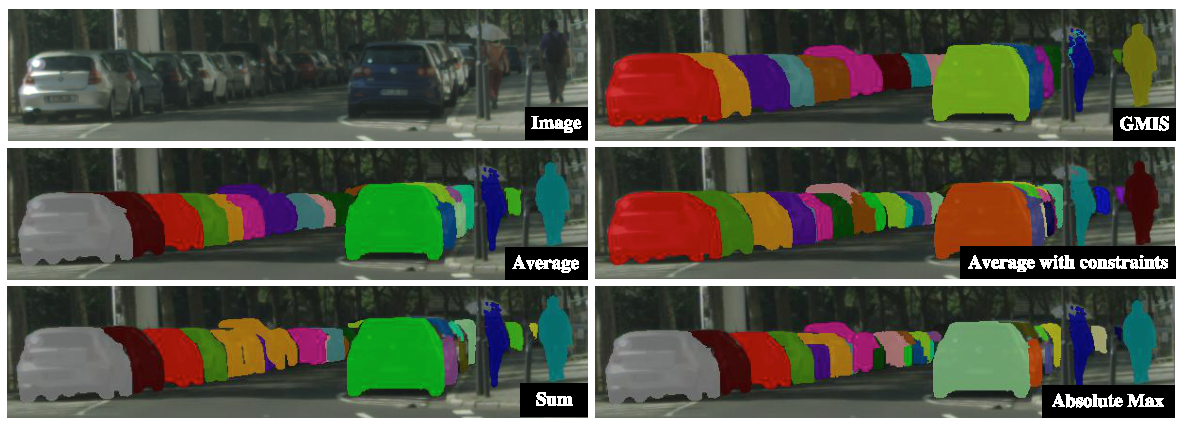
\includegraphics[width=\textwidth]{./figs/cityscapes_compare_6.pdf} % left bottom right top
\caption{Visual results given by different \algname{} linkage criteria on a crop of a CityScapes image from the \emph{validation} set.}\label{fig:cityscapes}
\end{minipage}
\end{figure}


